% DOC SETTINGS ===================================
\documentclass{article}
\usepackage[utf8]{inputenc}
\usepackage{fancyhdr}
\pagestyle{fancy}
\usepackage{geometry}
 \geometry{
 a4paper,
 total={170mm,257mm},
 left=20mm,
 top=25mm,
 }
\fancyheadoffset{0mm}
\lhead{ECE3544 HW2}
\rhead{Kavin Thirukonda 2021}
\usepackage{karnaugh-map}
\usepackage{circuitikz}
\usepackage{steinmetz}
\usepackage{listings}
\usepackage{xparse}
\usepackage{xstring}
\usepackage{circuitikz}
\usetikzlibrary{positioning, fit, calc}
\usepackage{mathtools}  
\mathtoolsset{showonlyrefs} 
\usetikzlibrary{circuits.logic.US,circuits.logic.IEC, positioning}
\cfoot{}
% DOC SETTINGS ===================================
\begin{document}
\begin{enumerate}
    \item Use a truth table to show that the “distributive theorem for Boolean algebra: $[(x+y) \cdot (x+z) = x + y \cdot z]$"
    \begin{center}
        \begin{tabular}{c|c|c|c}
        x & y & z & $(x+y) \cdot (x+z)$\\
        \hline
        0 & 0 & 0 & 0\\
        0 & 0 & 1 & 0\\
        0 & 1 & 0 & 0\\
        0 & 1 & 1 & 1\\
        1 & 0 & 0 & 1\\
        1 & 0 & 1 & 1\\
        1 & 1 & 0 & 1\\
        1 & 1 & 1 & 1
    \end{tabular}
    $\Rightarrow$
    \begin{tabular}{c|c|c|c}
        x & y & z & $x + y \cdot z$\\
        \hline
        0 & 0 & 0 & 0\\
        0 & 0 & 1 & 0\\
        0 & 1 & 0 & 0\\
        0 & 1 & 1 & 1\\
        1 & 0 & 0 & 1\\
        1 & 0 & 1 & 1\\
        1 & 1 & 0 & 1\\
        1 & 1 & 1 & 1
    \end{tabular}
    \end{center}
    \item Use a Karnaugh map to find a minimal SOP expression for the function F(a,b,c,d) = $\Sigma$(0,2,6,7,8,9,10,14,15)
    \begin{center}
        \begin{karnaugh-map}[4][4][1][$AB$][$CD$]                                        
          \minterms{0,2,6,7,8,9,10,14,15}
          \maxterms{1,3,4,5,11,12,13}
          \implicant{7}{14}
          \implicantcorner{0}{10}
          \implicant{8}{9}
        \end{karnaugh-map}
        
        f(a, b, c, d) = b'd' + bc + ab'c'
    \end{center}
    \item Implement a hazard free circuit for F(a, b, c) =  $\Sigma$(0, 2, 3, 4).  In your circuit, show which term(s) are required for the minimal implementation and which term(s) are required to remove the hazard
    \begin{center}
        \begin{karnaugh-map}[4][2][1][$AB$][$C$]
            \minterms{0, 2, 3, 4}
            \maxterms{1, 5, 6, 7}
            \implicant{0}{4}
            \implicant{3}{2}
            \implicantedge{0}{0}{2}{2}
        \end{karnaugh-map}
        
        f(a, b, c) = a'b' + c'b' + c'a
        \begin{center}
            \boxed{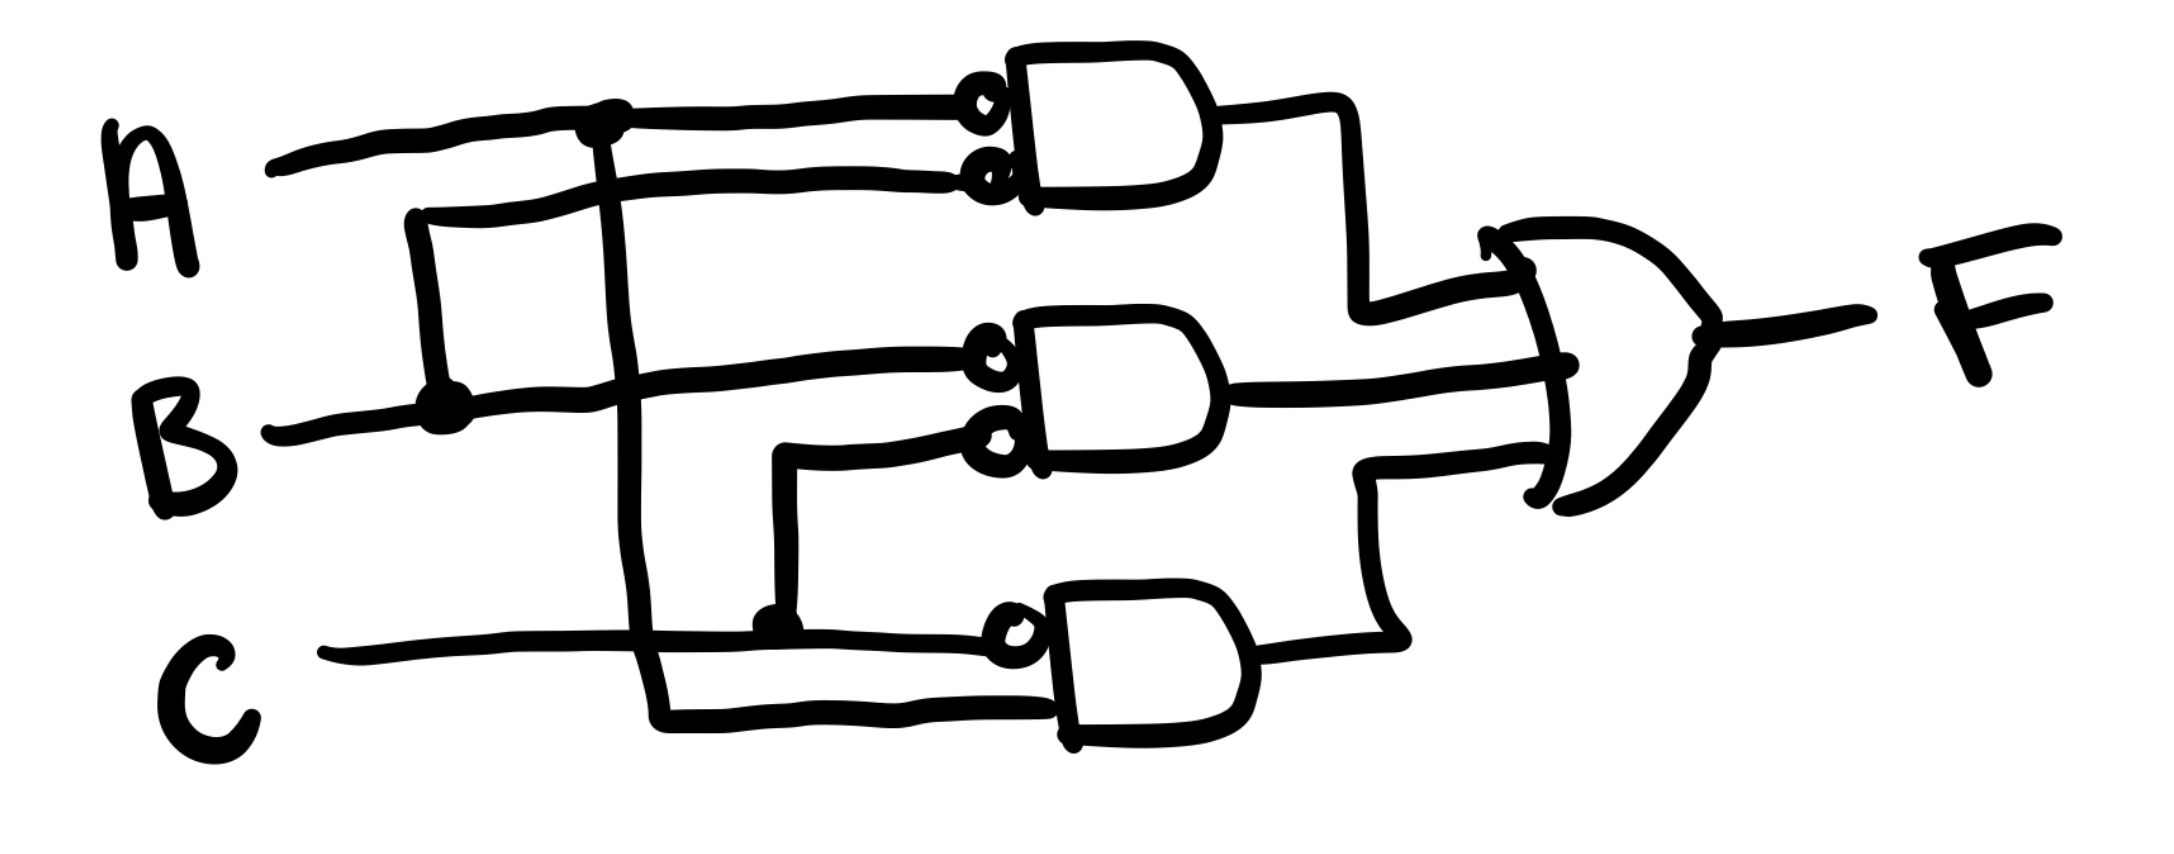
\includegraphics[width = .5\textwidth]{p3.png}}
            
            The c'b' term is required to remove the hazard
        \end{center}
    \end{center}
    \newpage
    \item For the function F(A, B, C, D) = $\Sigma$(1, 2, 3, 4, 5, 6, 10, 11, 13)
    \begin{enumerate}
        \item Map the function using the Karnaugh map shown below. Then use the map to identify the prime implicants of F.
        \begin{center}
        \begin{karnaugh-map}[4][4][1][$AB$][$CD$]                                        
          \minterms{1, 2, 3, 4, 5, 6, 10, 11, 13}
          \maxterms{0,7,8,9,12,14,15}
          \implicantedge{4}{4}{6}{6}
          \implicantedge{3}{2}{11}{10}
          \implicant{5}{13}
          \implicant{1}{3}
          \implicant{4}{5}
          \implicant{1}{5}
        \end{karnaugh-map}
        \end{center}
        \item Which  of  the  prime  implicants  of  F  (if  any)  are  essential  prime implicants?
        \begin{center}
        \begin{karnaugh-map}[4][4][1][$AB$][$CD$]                                        
          \minterms{1, 2, 3, 4, 5, 6, 10, 11, 13}
          \maxterms{0,7,8,9,12,14,15}
          \implicantedge{4}{4}{6}{6}
          \implicantedge{3}{2}{11}{10}
          \implicant{5}{13}
          \implicant{1}{3}
        \end{karnaugh-map}
        \end{center}
        \item If any of the minterms remain uncovered, which of the non-essential prime implicants cover those minterms minimally?
        \begin{center}
        \begin{karnaugh-map}[4][4][1][$AB$][$CD$]                                        
          \minterms{1, 2, 3, 4, 5, 6, 10, 11, 13}
          \maxterms{0,7,8,9,12,14,15}
          \implicantedge{4}{4}{6}{6}
          \implicantedge{3}{2}{11}{10}
          \implicant{5}{13}
          \implicant{1}{3}
        \end{karnaugh-map}
        
        None remain uncovered
        \end{center}
        \item Express a minimal two-level SOP implementation for F.
        \begin{center}
            f(a, b, c, d) = b'c + bc'd + a'b'd + a'bd'
        \end{center}
    \end{enumerate}
    \newpage
    \item Consider the following two functions:
    \begin{center}
        X(a, b, c, d) = (a + b’)(c + (bd))
        
        Y(a, b, c, d) = (a(c+d’)) + (c+(bd))
    \end{center}
    \begin{enumerate}
        \item Show how  to implement the functions simultaneously using only two input NAND gates and inverters in a multilevel circuit. Share any sub-expressions that  you  can  when  implementing  the  circuit.(Make  ONE  circuit  for  X \& Y (combined), not two circuit blocks)
        \begin{center}
            \boxed{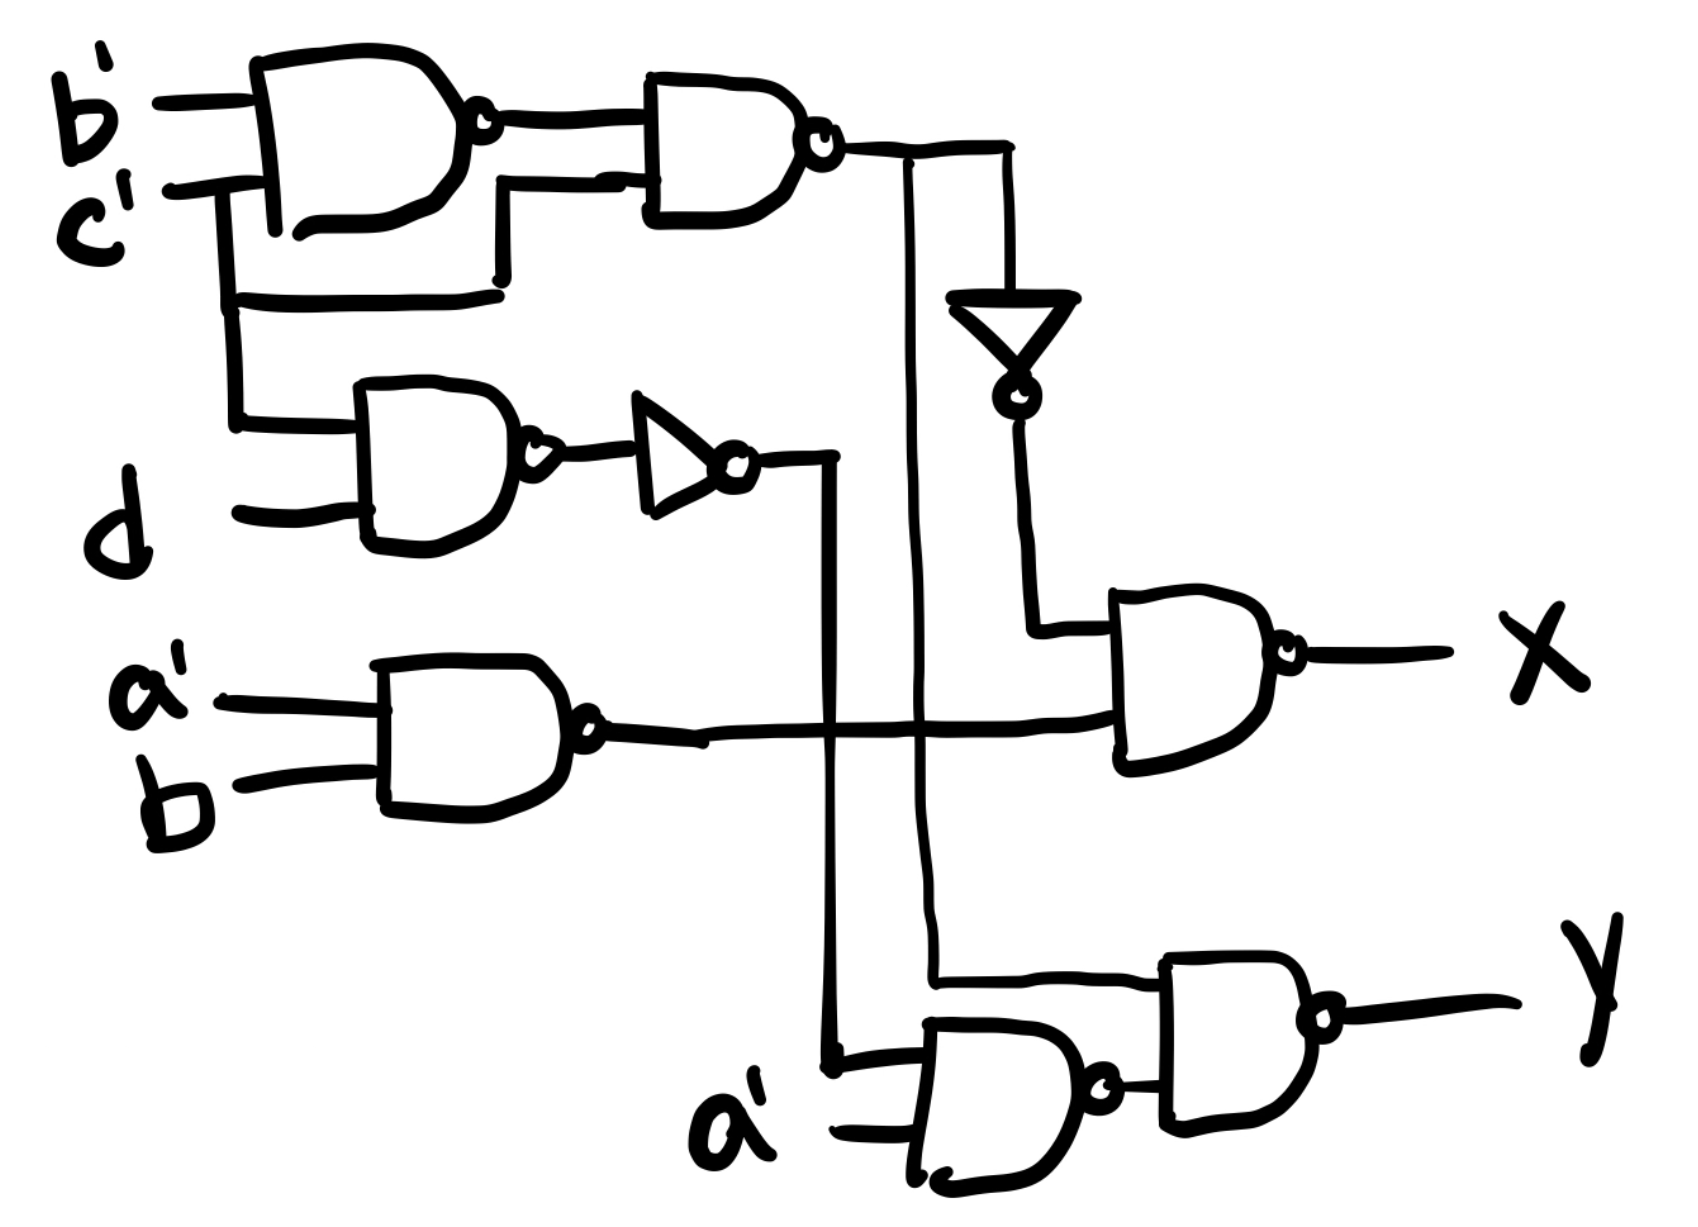
\includegraphics[width = .4\textwidth]{p5.png}}
        \end{center}
        \item Find the minimized two-level SOP expressions for X and Y. 
        \begin{center}
        \begin{karnaugh-map}[4][4][1][$A_XB_X$][$C_XD_X$]       \minterms{2, 3, 13, 15, 14, 11, 10}
          \maxterms{0, 1, 4,5,6,7,8,9,12}
          \implicant{13}{15}
          \implicant{15}{10}
          \implicantedge{3}{2}{11}{10}
        \end{karnaugh-map}
        \begin{karnaugh-map}[4][4][1][$A_YB_Y$][$C_YD_Y$]         \minterms{2,3,5,6,7,8,10,11,12,13,14,15}
            \maxterms{0,1,4,9}
            \implicant{3}{10}
            \implicant{5}{15}
            \implicantedge{12}{8}{14}{10}
        \end{karnaugh-map}
        \end{center}
        \item Implement  the  minimized  SOP expressions  using  only  two  input NAND  gates  and  inverters.  Share  any  sub-expressions  that  you  can  when implementing the circuit.
        \begin{center}
            \boxed{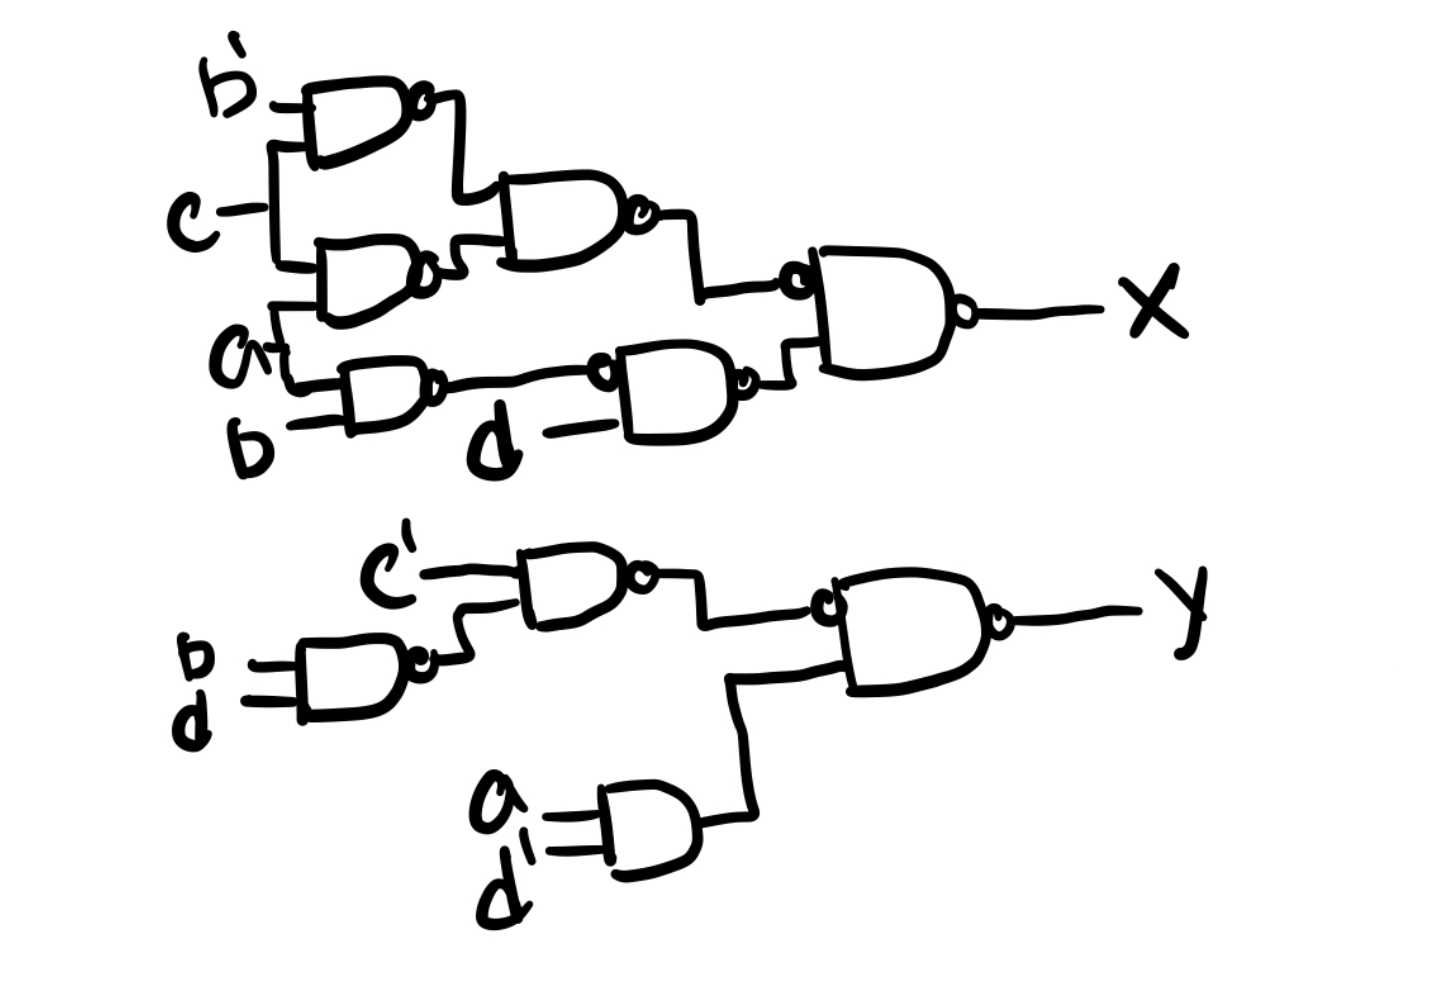
\includegraphics[width = .5\textwidth]{p52.png}}
        \end{center}
        \item Compare your circuits a and c in terms of gate counts for NANDs and inverters.  Briefly explain which circuit you would rather build.
        \begin{center}
            I would rather build the circuit in (a) because it takes less transistors overall because it reused circuits from both expressions to come up with a final value for each while the optimized version did not have this.
        \end{center}
    \end{enumerate}
\end{enumerate}
\end{document}
